\documentclass{article}
\usepackage{graphicx} % Required for inserting images
\usepackage[english]{babel}
\usepackage{amsthm}
\usepackage{amsmath}
\usepackage{amsfonts}
\usepackage{tikz}
\usetikzlibrary{matrix}

\title{MMath project}
\author{Saxon Supple }
\date{January 2024}

\begin{document}

\maketitle

\section{Proof of the Borsuk-Ulam theorem with cohomology}

\textrm{(Hatcher section 3.2 exercise 3) \\}
We begin with the following lemma.\\
\newtheorem{lemma}{lemma}
\begin{lemma}
There is no map $\mathbb{R} P^n$$\rightarrow$$\mathbb{R} P^m$ inducing a nontrivial map $H^1(\mathbb{R} P^m;\mathbb{Z}_2)\rightarrow H^1(\mathbb{R} P^n;\mathbb{Z}_2)$ if $n>m$.
\end{lemma}
\begin{proof}
Let $x_n$ and $x_m$ be the generators of $H^1(\mathbb{R} P^n;\mathbb{Z}_2)$ and $H^1(\mathbb{R} P^m;\mathbb{Z}_2)$ respectively.

\[H^1(\mathbb{R} P^n;\mathbb{Z}_2)\cong \mathbb{Z}_2\] 
\[H^*(\mathbb{R} P^n;\mathbb{Z}_2)\cong \mathbb{Z}_2[x]/<x^{n+1}>\] 

Let $f:\mathbb{R} P^n\rightarrow\mathbb{R} P^m $ be such a map so that $f^*(x_m)=x_n$.
Then since $f^*$ is a homomorphism on the cup product structure, $f^*(0)=f^*(x_m^{m+1})=f^*(x_m)^{m+1}=x_n^{m+1}=0$, requiring $m \geq n$. The result follows by contraposition.
\end{proof}

\begin{lemma}
Given any continuous map $f:\mathbb{R}P^n\rightarrow \mathbb{R}P^m$ with $n>m\geq 0$, $f_*:\pi_1(\mathbb{R}P^n)\rightarrow \pi_1(\mathbb{R}P^m)$ is trivial.
\end{lemma}
\begin{proof}
 $f^*:H^1(\mathbb{R}P^m;\mathbb{Z}_2)\rightarrow H^1(\mathbb{R}P^n;\mathbb{Z}_2)$ is dual to $f_*:H_1(\mathbb{R}P^n;\mathbb{Z}_2)\rightarrow H_1(\mathbb{R}P^m;\mathbb{Z}_2)$ which is equal to $f_*:\pi_1(\mathbb{R}P^n)\rightarrow \pi_1(\mathbb{R}P^m)$ by the Hurewicz theorem and the fact that $\pi_1(\mathbb{R}P^k)$ is abelian. Thus $f_*$ is trivial by the above result.
\end{proof}

We are now able to prove the main theorem.
\newtheorem{theorem}{theorem}
\begin{theorem}
\textbf{Borsuk-Ulam theorem:} For integers $n>m\geq 0$ there is no continuous map $\phi:S^n\rightarrow S^m$ which is antipode preserving, meaning $\phi(-x)=-\phi(x)$ for all $x$.
\end{theorem}
\begin{proof}
Suppose that there exists a continuous antipode preserving map $\phi:S^n\rightarrow S^m$. Define $\psi:\mathbb{R}P^n\rightarrow \mathbb{R}P^m$ by $\psi([x])=[\phi(x)]$. $\psi$ is well-defined since $x\sim y \implies x=\pm y \implies \phi(x)=\pm\phi(y) \implies \phi(x)\sim\phi(y)$. $\psi$ is also continuous by the universal property of quotients for the quotient map $p:S^k\rightarrow \mathbb{R}P^k$.
Fix $x\in S^n$ and let $y=\phi(x)$. $\psi_*:\pi_1(\mathbb{R}P^n,[x])\rightarrow \pi_1(\mathbb{R}P^m,[y])$ is trivial by the above lemma, so has a unique lift $\psi':(\mathbb{R}P^n,[x])\rightarrow (S^m,y)$ under the covering map $p$ by the ultimate lifting theorem. This gives a commutative diagram

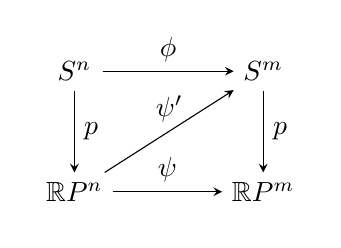
\begin{tikzpicture}
  \matrix (m) [matrix of math nodes,row sep=3em,column sep=4em,minimum width=2em] {
     S^n & S^m \\
     \mathbb{R}P^n & \mathbb{R}P^m \\};
  \path[-stealth]
    (m-1-1) edge node [right] {$p$} (m-2-1)
            edge  node [above] {$\phi$} (m-1-2)
    (m-2-1.east|-m-2-2) edge  node [above] {$\psi$} (m-2-2)
    (m-1-2) edge node [right] {$p$} (m-2-2)
            (m-2-1) edge  node [above]{$\psi'$} (m-1-2);
\end{tikzpicture}
\\
$\psi' \circ p$ and $\phi$ are both lifts of $\psi \circ p$ and both map $x\mapsto y$ so $\phi = \psi'\circ p$ by uniqueness. But then $\psi'(p(-x))=\psi'([x])=y=\phi(x)$, contradicting $\phi(-x)=-y$.
\end{proof}

\end{document}
